\documentclass[conference]{IEEEtran}
\usepackage[english]{babel}
\usepackage[utf8]{inputenc}
\usepackage{amsmath}
\usepackage{amsfonts}
\usepackage{graphicx}
\usepackage[colorinlistoftodos]{todonotes}
\usepackage{algorithm,algorithmicx}
\usepackage{algpseudocode}
\usepackage{blindtext, graphicx}
\usepackage{comment}
\usepackage{hyperref}
\usepackage{caption}
\usepackage{float}
\usepackage[demo]{graphicx}
\usepackage{subfig}
%
\usepackage[absolute,showboxes]{textpos}

\usepackage{rotating}
\definecolor{Gray}{rgb}{0.88,1,1}
\definecolor{Gray}{gray}{0.85}
\definecolor{Blue}{RGB}{0,29,193}
\definecolor{lightgray}{gray}{0.8}
\definecolor{darkgray}{gray}{0.6}
\definecolor{LightGray}{gray}{0.975}

\usepackage{multirow}
\usepackage{tcolorbox}% http://ctan.org/pkg/tcolorbox
\definecolor{mycolor}{rgb}{0.122, 0.435, 0.698}% Rule colour
\makeatletter
\newcommand{\mybox}[1]{%
  \setbox0=\hbox{#1}%
  \setlength{\@tempdima}{\dimexpr\linewidth}%
  \begin{tcolorbox}[colframe=mycolor,boxrule=0.5pt,arc=4pt,
      left=6pt,right=6pt,top=6pt,bottom=6pt,boxsep=0pt,width=\@tempdima]
    #1
  \end{tcolorbox}
}
\makeatother

\usepackage[svgnames]{xcolor}
\usepackage[framed]{ntheorem}
\usepackage{framed}
\usepackage{tikz}
\usetikzlibrary{shadows}
%\newtheorem{Lesson}{Lesson}
\theoremclass{Lesson}
\theoremstyle{break}

% inner sep=10pt,
\tikzstyle{thmbox} = [rectangle, rounded corners, draw=black,
  fill=Gray,  drop shadow={fill=black, opacity=1}]
\newcommand\thmbox[1]{%
  \noindent\begin{tikzpicture}%
  \node [thmbox] (box){%
\begin{minipage}{.94\textwidth}%    
      \vspace{-3mm}#1\vspace{-3mm}%
    \end{minipage}%
  };%
  \end{tikzpicture}}

\let\theoremframecommand\thmbox
\newshadedtheorem{lesson}{Result}

%\hyphenation{op-tical net-works semi-conduc-tor}


\begin{document}

\title{\textbf{Taming Topic Instability For Reasoning Over Unstructured Data in Software Engineering}}


\author{

\IEEEauthorblockN{Amritanshu Agrawal}
\IEEEauthorblockA{Computer Science, NCSU\\
Raleigh, North Carolina\\
aagrawa8@ncsu.edu}
\and
\IEEEauthorblockN{Tim Menzies}
\IEEEauthorblockA{Computer Science, NCSU\\
Raleigh, North Carolina\\
tim.menzies@gmail.com}
\and
\IEEEauthorblockN{Wei Fu}
\IEEEauthorblockA{Computer Science, NCSU\\
Raleigh, North Carolina\\
wfu@ncsu.edu}

}

% make the title area
\maketitle


\begin{abstract}
%\boldmath
Topic Modeling has been widely used to identify patterns in a corpus across various fields. The Latent Dirichlet Allocation (LDA) algorithm is a widely used topic modeling algorithm which in practice is called using its defaults. We report that these defaults can lead to highly misleading results in Software Engineering (SE). It is very important to generate stable topics using the Non-Deterministic LDA method. But one of the curse is setting the right parameters that control the LDA. We ran differential evolution (DE) as an optimizer to explore the tuning space (as a first step) then tested it against the default parameter settings. We found that these tunings were remarkably simple, and took hundreds, not thousands of evaluations to obtain very good results. Since the improvements are so large, and (2) the tuning is so simple, that many industries, who are using LDA, should change the standard methods for better throughput and accuracy of their products. The implication for other kinds of topic modeling algorithms is now an open and pressing issue.
\end{abstract}

\begin{IEEEkeywords}
Topic modeling, Stability, LDA, tuning, differential evolution.
\end{IEEEkeywords}


\IEEEpeerreviewmaketitle


\section{Introduction}
\label{sect: intro}
In the 21st century, we have now access amount of data about Software Engineering. Most of these data is in an unstructured format~\cite{nadkarni2014structured}. According to International Data Corporation (IDC), shown in figure \ref{fig: data}, this number is about 1600 Exabytes. Unstructured data does not have a pre-defined data model and is typically text-heavy. Finding insights among unstructured text is extremely difficult unless we can search, characterize, and classify the text data in a meaningful way.

\begin{figure}[!htpb]
  \captionsetup{justification=centering}
  \includegraphics[width=\linewidth]{./fig/data.png}
  \caption{Data Growth 2005-2015}
  \label{fig: data}
\end{figure}

One of the common techniques for finding related topics within unstructured text (an area called topic modeling) is Latent Dirichlet Allocation (LDA) as introduced in the next section. It is usually used with off-the-shell default parameters. But what we found is due to the algorithms non-deterministic behaviour, the topics generated are not stable. In the coming sections, we will be explaining the reason for this non-deterministic behaviour and possible workarounds given by other researchers to mitigate stability of LDA to some extent.

There are various libraries which provide LDA implementation and each library comes with a set of parameters. It is very impractical to get the right combination of parameters due to larger search space. To tackle the above problem, we observed that the parameters taken by LDA can be tuned. In the next coming sections, we will show that many researchers have agreed to the idea of using different configurations for generating topics using LDA. But, we have seen rare work done when it comes to tune the important parameters of LDA for getting stable topics. Most people have went ahead with LDA’s default parameters and have not searched the whole configurations space.

To tackle the problem of how to tune, we have seen that one of the simplest \textit{\textbf{multiobjective optimizers (differential evolution}}~\cite{storn1997differential}) works very well for tuning in certain kinds of software analytics~\cite{fu2016tuning}. There has been success stories where DE has helped in tuning the parameters~\cite{fu2016tuning, bazi2014differential, chiha2012tuning}. Prior to this work, our intuition was that tuning would change the behavior of LDA, to some degree. Also, we suspected that tuning would take so long time and be so CPU intensive that the benefits gained would not be worth the effort. We have found large instability in 2 data miners, namely, defect predictors and LDA. Results have shown that we can contain the instability to a large extent using Differential Evolution (DE). So, this makes us wonder Search-Based Software Engineering (SBSE) techniques can help us.

The results of this paper show that the above points are false since:
\begin{enumerate}
  \item Tuning LDA is remarkably simple;
  \item And can dramatically improve stability in the topic generation.
\end{enumerate}

We can say that now, we can mitigate instability of non-deterministic LDA. We are talking about model instability itself rather than results instability. Many industries, working on a product development in text analytics have been widely using LDA. This gives them a chance to incorporate better throughput and accuracy in their product. Menzies et al.~\cite{menzieslocal} showed how model instability can give rise to different effort estimations across various projects.

Those results were found by exploring six research questions:
\begin{itemize}
    \item \textbf{RQ1}: \textit{Do the default settings lead to misleading results?} We will show that topics generated with the default settings are misleading as stability scores start to drop after top 5 terms, which is the basis to define a particular topic generated from LDA.
    \item \textbf{RQ2}: \textit{Does tuning improve the stability scores of LDA?} In our work, we will show dramatic improvement in the stability scores with the tuned parameters rather than going for default parameters.
    \item \textbf{RQ3}: \textit{Does different data need different configurations to make LDA stable? Does it change some predefined parameter values of LDA?} We will show that different sets of configurations are found out by DE. For one of the results, we showed that we need topic size of less than 30 rather than 67~\cite{garousi2016citations}.
    \item \textbf{RQ4}: \textit{Is tuning easy?} We have seen that one of the simpler multiobjective optimizers (differential evolution~\cite{storn1997differential}) works very well for tuning in major software analytics.
    \item \textbf{RQ5}: \textit{Is tuning impractically slow?} We achieved dramatic improvements in the stability scores of LDA in less than 300 evaluations (!); i.e., very quickly.
    \item \textbf{RQ6}: \textit{Should data miners be used “off-the-shelf” with their default tunings?} Wei et al.~\cite{fu2016tuning} showed that for defect prediction from static code measures, their answer is an emphatic “no”. And we also say that for LDA, it is a “no”. 
\end{itemize}

Topic Modeling have been used in various spheres of SE. Sun et al. reported a survey of LDA's usage to support various SE tasks between 2003 and 2015~\cite{sun2016exploring}. The number of papers published across top major conferences and journals are listed in figure \ref{fig: venues}. The survey in figure \ref{fig: survey} show that there is an increasing concern in this area.

\begin{itemize}
    \item Topic modeling is applied in various SE tasks, including source code comprehension, feature location, software defects prediction, developer recommendation, traceability link recovery, re-factoring, software history comprehension, software testing and social software engineering.

\begin{figure}[!htpb]
  \captionsetup{justification=centering}
  \includegraphics[width=\linewidth]{./fig/venues.png}
  \caption{Survey Venue and Statistics}
  \label{fig: venues}
\end{figure}

\begin{figure}[!htpb]
  \captionsetup{justification=centering}
  \includegraphics[width=\linewidth]{./fig/survey.png}
  \caption{The distribution of the papers published in different years}
  \label{fig: survey}
\end{figure}

    \item There are works in Requirements Engineering where it was necessary to analyze the text and come up with the important topics~\cite{asuncion2010software, thomas2014studying, massey2013automated}.
    \item People have used topic modeling in prioritizing test cases, and identifying the importance of test cases~\cite{hemmati2015prioritizing, zhang2015inferring, yang2015predicting}.
    \item Increasingly, it has also become very important to have automated tools to do a Systematic Literature Review (SLR)~\cite{tsafnat2014systematic}. We found these papers~\cite{restificar2012inferring,alreview,marshall2013tools} who have used clustering algorithms (topic modeling) to do SLR.
\end{itemize}

Since topic modeling has been widely used in various spheres of SE, and it is really important to generate stable topics. Prior Papers who reports LDA may have been severely compromised. This gives all of us the motivation of generating stable topics in software engineering which will make product development faster, cheaper and accurate.

\section{Previous Work}

Are the impacts of instability in LDA addressed in the text analytics? To answer that question, in April 2016, we searched scholar.google.com for the conjunction of “lda” and “topics” or “stable” or “unstable” or “coherence”. At the time of writing this paper, we got 475 results. We selected for papers since 2012, we got to 189 results. After discarding the non-SE papers, we read over this sample of 57 highly-cited SE text analytics papers. 28 papers talk about instability in LDA (more details can be found at \href{https://goo.gl/Bpc6Vb}{\textit{https://goo.gl/Bpc6Vb}}). Also, we found in that sample was that only two authors acknowledged the impact of tunings. About 35\% papers in our sample did not adjust the “off-the-shelf” configuration of the LDA. Among the other 65\%, 83\% papers, explored the configurations space with brute force. Their was not an effective and faster way of choosing the right set of parameters. Those papers, which accepted the problem of instability in LDA, came to some conclusions which can be found in Table \ref{tb:survey}. The literature review for rest of the papers are categorized in the following subsections.
\begin{center}
\begin{table*}[!htb]
{\small
\hfill{} 
\begin{tabular}{|c|c|c|c|c|c|}
        \hline 
        \multicolumn{1}{|p{1.3cm}|}{\centering \textbf{Reference} \\\textbf{ID}} & \textbf{Citations} & \multicolumn{1}{|p{1.3cm}|}{\centering \textbf{Mentions} \\\textbf{instability} \\\textbf{in LDA?}} & \multicolumn{1}{|p{2cm}|}{\centering \textbf{Talks} \\\textbf{about} \\\textbf{using} \\\textbf{off the} \\\textbf{shell} \\\textbf{parameters}?} & \multicolumn{1}{|p{1cm}|}{\centering \textbf{Does} \\\textbf{tuning?}} & \textbf{\textbf{Conclusion}}\\ [0.5ex]
        \hline
        ~\cite{rao2011retrieval} & 112 & Y & Y & N  & \begin{tabular}[c]{@{}l@{}}Explored Configurations without any explanation\end{tabular} \\ [0.5ex]
        \hline
        ~\cite{oliveto2010equivalence} & 108 & Y & Y & N & \begin{tabular}[c]{@{}l@{}}Explored Configurations without any explanation\\ Reported their results using multiple experiments\end{tabular} \\ [0.5ex]\hline
        ~\cite{barua2014developers} & 96 & Y & Y & N  & \begin{tabular}[c]{@{}l@{}}Explored Configurations without any explanation \\Choosing right set of parameters is a difficult task\end{tabular} \\ [0.5ex]
        \hline
        ~\cite{panichella2013effectively} & 75 & Y & Y & Y  & \begin{tabular}[c]{@{}l@{}}Uses GA to tune parameters. They determine the \\near-optimal configuration for LDA in the context \\of only some important SE tasks\end{tabular} \\ [0.5ex]
        \hline
        ~\cite{galvis2013analysis} & 61 & Y & Y & N  & \begin{tabular}[c]{@{}l@{}}Explored Configurations without any explanation\end{tabular} \\ [0.5ex]
        \hline
        ~\cite{hindle2011automated} & 45 & Y & Y & N  & \begin{tabular}[c]{@{}l@{}}They validated the topic labelling techniques using \\multiple experiments.\end{tabular} \\ [0.5ex]
        \hline
        ~\cite{guzman2014users} & 44 & Y & Y & N  & \begin{tabular}[c]{@{}l@{}}Explored Configurations without any explanation\end{tabular} \\ [0.5ex]
        \hline
        ~\cite{thomas2011mining} & 44 & Y & Y & N  & \begin{tabular}[c]{@{}l@{}}Open issue to choose optimal parameters\end{tabular} \\ [0.5ex]
        \hline
        ~\cite{chen2012explaining} & 35 & Y & Y & N  & \begin{tabular}[c]{@{}l@{}}Choosing the optimal number of topics is difficult\end{tabular} \\ [0.5ex]
        \hline
        ~\cite{thomas2014studying} & 35 & Y & Y & N  & \begin{tabular}[c]{@{}l@{}}Explored Configurations without any explanation\end{tabular} \\ [0.5ex]
        \hline
        ~\cite{thomas2014static} & 31 & Y & Y & N  & \begin{tabular}[c]{@{}l@{}}Choosing right set of parameters is a difficult task\end{tabular} \\ [0.5ex]
        \hline
        ~\cite{bajracharya2009mining} & 29 & Y & Y & N  & \begin{tabular}[c]{@{}l@{}}Explored Configurations without any explanation \\and accepted to the fact their results were better \\because of the corpus they used\end{tabular} \\ [0.5ex]
        \hline
        ~\cite{lohar2013improving} & 27 & Y & Y & Y  & \begin{tabular}[c]{@{}l@{}}Explored Configurations using LDA-GA\end{tabular} \\ [0.5ex]
        \hline
        ~\cite{linares2013exploratory} & 20 & Y & Y & N  & \begin{tabular}[c]{@{}l@{}}In Future, they planned to use LDA-GA\end{tabular} \\ [0.5ex]
        \hline
        ~\cite{koltcov2014latent} & 15 & Y & Y & N  & \begin{tabular}[c]{@{}l@{}}Explored Configurations without any explanation\end{tabular} \\ [0.5ex]
        \hline
        ~\cite{hindle2012relating} & 13 & Y & Y & N  & \begin{tabular}[c]{@{}l@{}}Explored Configurations without any explanation \\(Just with no. of topics)\end{tabular} \\ [0.5ex]
        \hline
        ~\cite{grant2013using} & 13 & Y & Y & N  & \begin{tabular}[c]{@{}l@{}}Their work focused on optimizing LDA’s topic \\count parameter\end{tabular} \\ [0.5ex]
        \hline
        ~\cite{fu2015automated} & 6 & Y & Y & N  & \begin{tabular}[c]{@{}l@{}}Explored Configurations without any explanation.\\ Choosing right set of parameters is a difficult task\end{tabular} \\ [0.5ex]
        \hline
        ~\cite{garousi2016citations} & 5 & Y & Y & N  & \begin{tabular}[c]{@{}l@{}}Explored Configurations without any explanation\end{tabular} \\ [0.5ex]
        \hline
        ~\cite{le2014predicting} & 5 & N & Y & N  & \begin{tabular}[c]{@{}l@{}}Explored Configurations without any explanation\end{tabular} \\ [0.5ex]
        \hline
        ~\cite{nikolenko2015topic} & 3 & Y & Y & N  & \begin{tabular}[c]{@{}l@{}}They improvised LDA into ISLDA which gave \\stability across different runs\end{tabular} \\ [0.5ex]
        \hline
        ~\cite{sun2015msr4sm} & 2 & Y & Y & Y  & \begin{tabular}[c]{@{}l@{}}Explored Configurations using LDA-GA\end{tabular} \\ [0.5ex]
        \hline
        ~\cite{chen2016topic} & 0 & N & Y & N  & \begin{tabular}[c]{@{}l@{}}Explored Configurations without any explanation. \\Choosing right set of parameters is a difficult task\end{tabular} \\ [0.5ex]
        \hline
        ~\cite{yang2015improving} & 2 & Y & N & N  & \begin{tabular}[c]{@{}l@{}}Uses modified frameworks of LDA. This is for \\classified datasets.\end{tabular} \\ [0.5ex]
        \hline
\end{tabular}
}
\hfill{}
\newline
\caption{Literature Survey}
\label{tb:survey}
\end{table*}
\end{center}
\subsection{Problems with LDA}
\label{sect: problems}

\begin{itemize}
    \item In LDA, learning the various distributions is a problem of Bayesian inference. It also uses the alternative inference techniques like Gibbs sampling~\cite{wei2006lda, griffiths2004finding} and expectation propagation (VEM)~\cite{minka2002expectation}. These techniques gave rise to non deterministic ways which are responsible for the instability in the topic modeling. Different inference techniques in LDA try to maximize the resulting lower bound on the log likelihood~\cite{blei2003latent}. The expected complete log likelihood of the data can have many local maximas, which leads to different distributions and in turn leads to instability in the output. The distributions which are found with the help of LDA, resulting from the same dataset with the same vocabulary and model parameters, any differences between them are entirely due to the randomness in inference techniques~\cite{koltcov2014latent}. This randomness affects perplexity variations, word and document ratios. There is a problem of finding the optimal number of clusters, but different configuration parameters may lead us to the stable topics.
    \item The topics learned by LDA sometimes are difficult to interpret by end users~\cite{yang2015improving, panichella2013effectively}. We want topics to be finer grained (more number of topics) or coarse grained (less number of topics) according to the use case. Rationality about the topics instability is important if an industry is using topic modeling in all their use cases~\cite{lau2014machine, o2015analysis}. We do not want vaguely defined topics.
    \item Online learning~\cite{hoffman2010online} for LDA uses constant memory requirements and empirically converges faster than batch collapsed Gibbs sampling. However, it still requires a full pass through the entire corpus each iteration. It can therefore be slow to apply to very large datasets, and is not naturally suited to settings where new data is constantly arriving. New data arriving can induce more randomness in the inference techniques.
    \item We observed that this is just not happening with only particular programming language or particular library. This instability is happening irrespective of the tools in which LDA has been implemented. Some of the papers mentioned using GibbsLDA++ written in C++ and they observed the same instability~\cite{lukins2008source, tian2009using, guzman2014users}. Some papers mentioned about using Python implementation of LDA and observed the same instability~\cite{guzman2014users}. LDA implemented in JAVA language produced the same incoherent topics~\cite{martin2015app, hindle2011automated}. And, we observed this problem is in the Scikit-Learn version of LDA, implemented in Python, as well as Spark Mllib library.
\end{itemize}

\subsection{Tuning: Important and Ignored}
\label{sect: tuning}

This section argues that tuning is an under-explored software analytics. The impact of tuning is well understood~\cite{bergstra2012random}. Yet issues of tuning are rarely or poorly addressed in the data analytics literature. When we tune a data miner, what we are really doing is changing how a learner applies its heuristics. This means tuned data miners use different heuristics, which means they ignore different possible models, which means they return different models; i.e. how we learn changes what we learn.

Wei et al.~\cite{fu2016tuning} shows that only few authors acknowledged the impact of tunings. A few other papers did acknowledge that one data miner may not be appropriate for all data sets. Those papers tested different “off-the-shelf” data miners on the same data set. For
example, Elish et al.~\cite{elish2008predicting} compared support vector machines to other data miners for the purposes of defect prediction. Those papers tested different “off-the-shelf” data miners on the same data set. Wei et al.~\cite{fu2016tuning} showed that finding useful tunings is very easy. This result is both novel and unexpected. Learners are very amenable to tuning. Hence, they are also very amenable to significant performance improvements. Given the low number of evaluations required, they asserted that tuning should be standard practice for anyone using data miners.

\subsection{WorkAround to LDA Instability Problem}
\label{sect: solutions}

\subsubsection{\textbf{Unsupervised}}
\hfill

\noindent\fbox{
    \parbox[][][s]{\linewidth-0.35cm}{%
    \textbf{Solution 1}:
    To evaluate the stability of topics, most papers~\cite{maskeri2008mining, martin2015app, guzman2014users} manually accessed the topics and then used for further experiments. Some made use of Amazon Mechanical Turk to create gold-standard coherence judgements~\cite{lau2014machine}.
    }%
}

\mybox{This workaround will take a lot of manual effort and time which is not feasible for many. In the age of automation, we need an efficient way of making LDA stable.}

\noindent\fbox{
    \parbox[][][s]{\linewidth-0.35cm}{%
    \textbf{Solution 2}:
    Users have external knowledge regarding word correlation, which can be taken into account to improve the semantic coherence of topic modeling methods. SCLDA~\cite{yang2015improving} can handle different kinds of knowledge such as word correlation, document correlation, document label and so on. One advantage of SC\-LDA over existing methods is that it is very fast to converge.
    }%
}

\mybox{We do not have enough resources to have a user knowledge for the type of datasets we used, and that's the reason we are not using this solution to improve stability.}

\noindent\fbox{
    \parbox[][][s]{\linewidth-0.35cm}{%
    \textbf{Solution 3}:
    The most common parameters in the LDA are number of clusters (\textit{k}), number of iterations (\textit{n}), document topic prior ($\alpha$), and word topic prior ($\beta$). The other solution is tuning these parameters of LDA. Some researchers~\cite{panichella2013effectively, lohar2013improving, sun2015msr4sm} used Genetic Algorithm (GA) to tune the parameters and then using different configurations for LDA. Some people~\cite{galvis2013analysis, tian2009using} achieved higher stability by just increasing the number of cluster size.
    }%
}

\mybox{We found this to have better advantage than the other solutions based on the tuning work done by Wei~\cite{fu2016tuning}. And in our work, we have used this solution.}
 
%\end{lesson}


\subsubsection{\textbf{Supervised}}
\label{sub:supervised}
\hfill

\noindent\fbox{
    \parbox[][][s]{\linewidth-0.35cm}{%
    \textbf{Solution 3}:
    We found so many improvised frameworks of LDA namely, \textit{Labeled LDA}~\cite{ramage2009labeled}, \textit{Dirichlet Forest LDA}~\cite{andrzejewski2009incorporating}, \textit{Logic LDA}~\cite{andrzejewski2011framework}, \textit{Quad-LDA}~\cite{newman2011improving}, \textit{NMF-LDA}~\cite{xie2015incorporating}, \textit{Interactive Topic Modeling} (ITM)~\cite{hu2014interactive}, \textit{MRTF}~\cite{daume2009markov} and many more, helping in generating better stable topics.
    }%
}

\mybox{We will not be able to use any of the above supervised solutions as our datasets are not labeled. And all these frameworks work best with the classified datasets. This is going to be our future work which we will be addressing next.}

\subsection{Evaluation}
\label{sect: evaluation}
To evaluate the topics coherence or the cluster stability using LDA, there has been number of evaluation measures proposed. There is a direct approach, by asking people about topics, and an indirect approach by evaluating \textit{pointwise mutual information (PMI)}~\cite{lau2014machine, o2015analysis} between the topic words. PMI being an automatic method, we are not sure of exact details of it which made us to not use this measure. We could not use direct approach, due to resource limitation to ask an expert for the type of datasets we used.

\textit{Perplexity} is monotonically decreasing in the likelihood of the data, and is algebraically equivalent to the inverse of the geometric mean per-word likelihood. It shows how well topic-word and word-document distributions predict new test samples. The smaller the perplexity, the better (less uniform) is the LDA model. The usual trend is that as the value of perplexity drops, the number of topics should grow~\cite{koltcov2014latent}. But problem with perplexity is that the value of perplexity doesn't remain constant with different topic size and with dictionary sizes~\cite{koltcov2014latent, zhao2015heuristic}. A lot depend on the code implementation of perplexity and the type of datasets used. Since, we are using different implementations of LDA as well as different datasets, we are not using Perplexity as evaluation measure.

Many researchers~\cite{o2015analysis, galvis2013analysis} use Jaccard Similarity for evaluating stability. We define our measure similar to it. We say topics are stable, when there are $x$ times $n\%$ of terms overlap in a topic across $m$ runs. We can see an example of 5 terms overlap in figure \ref{fig: jaccard}. We take median of all the scores generated by evaluating topic. In this example, figure \ref{fig: jaccard}, median score is $1.0$ for each run. So overall median score comes out to be $1.0$. We always select top 10 terms within a topic suggested by some researchers~\cite{panichella2013effectively, lukins2010bug}. It makes sense to us that to have a successful topic model, each topic can be identified using top few terms. \textit{If we get different words then it can mean different topics which can put any product based on topic modeling at risk.}

To understand our results, we have defined some terminologies. We call the above median score as \textbf{\textit{Raw score}} which is $1.0$. This \textit{Raw Score} can come from tuning and untuned results defined similarly. We also define a \textbf{\textit{Delta Score}} which is the absolute difference between \textbf{Raw Score$_{tuned}$ $-$ Raw Score$_{untuned}$}.

%\begin{figure*}[H]
%  \captionsetup{justification=centering}
%  \includegraphics[width=\textwidth,height=4cm]{./fig/jaccard.png}
%  \caption{Example of 5 terms overlap and its evaluation score}
%  \label{fig: jaccard}
%\end{figure*}
\begin{figure}[!htpb]
  \captionsetup{justification=centering}
  \includegraphics[width=\linewidth]{./fig/jaccard.png}
  \caption{Example of 5 terms overlap across 4 runs and its stability score}
  \label{fig: jaccard}
\end{figure}

\subsection{Notes on LDA}
\label{sect: LDA}
Latent Dirichlet Allocation (LDA) is a generative statistical model that allows sets of observations to be explained by unobserved groups that explain why some parts of the data are similar. It learns the various distributions (the set of topics, their associated word probabilities, the topic of each word, and the particular topic mixture of each document) and is a problem of Bayesian inference.
%Regardless of the methods, all these attempts to fit the model to data using maximum likelihood. Lesser the likelihood, more the convergence of the model and expected to achieve better results. The perplexity, used by convention in topic modeling, is monotonically decreasing in the likelihood of the data.
The pseudocode for untuned LDA is shown in Algorithm 1 with the default set of parameters. In the following description, superscript numbers denote lines in the pseudocode. The data is shuffled everytime LDA is run$^{L5}$. Data is in the form of term frequency scores of each word per document. Shuffling is done in order  to  induce  maximum  variance  among  different  runs of LDA. Topics$^{L6}$ is a list of list which contains topics from all the different runs. A stability score is evaluated on every 10 runs, and this process is continued 10 times. At the end, median score is selected as the untuned final score$^{L3-L11}$.

\makeatletter
\algrenewcommand\ALG@beginalgorithmic{\footnotesize}
\algrenewcommand\algorithmiccomment[2][\normalsize]{{#1\hfill\(\triangleright\) #2}}
\makeatother
\renewcommand{\algorithmicrequire}{\textbf{Input:}}
\renewcommand{\algorithmicensure}{\textbf{Output:}}
\begin{algorithm}[!htb]
    %\scriptsize
    %\label{algo: untuned}
    \caption{Pseudocode for untuned LDA with Default Parameters}
    \begin{algorithmic}[1]
    %\label{algo: untuned}
    \Require $no. of terms$, $Data$
    \Ensure $Final\_Score$    
    \Function{ldascore}{ $no. of terms$, $Data$}
        \State $Score \leftarrow \emptyset$
        \For{$j = 0$ to 10}
            \For{$i = 0$ to 10}
                \State $data \leftarrow$ \textbf{shuffle}($Data$)
                \State $Topics$.append(lda($k=10$,$\alpha=none$,$\beta=none$ ))
            \EndFor
            \State $Score$.append($Overlap$(Topics, $no. of terms$, $l[0]$))
        \EndFor
        \State $Final\_Score \leftarrow $ median(Score)
        \State \textbf{return} $Final\_Score$
    \EndFunction
    %\medskip
    \end{algorithmic}
\end{algorithm}

\subsection{Tuning Algorithms}
\label{sect: tuning}

In section \ref{sect: solutions}, we talked about our reasoning why are we choosing tuning the parameters of LDA as the solution. Here is a list of optimizers used widely in research: simulated annealing~\cite{feather2002converging, menzies2007business}; various genetic algorithms~\cite{goldberg1979complexity} augmented by techniques such as differential evolution~\cite{storn1997differential}, tabu search and scatter search~\cite{glover1986general, beausoleil2006moss, molina2007sspmo, nebro2008abyss}; particle swarm optimization~\cite{pan2008particle}; numerous decomposition approaches that use heuristics to decompose the total space into small problems, then apply a response surface methods~\cite{krall2015gale, zuluaga2013active}. Of these, the simplest ones are simulated annealing (SA) and differential evolution (DE), each of which can be coded in less than a page of some highlevel scripting language. Our reading of the current literature is that there are more advocates for differential evolution than SA. For example, Vesterstrom and Thomsen~\cite{vesterstrom2004comparative} found DE to be competitive with particle swarm optimization and other GAs. DEs have been applied before for parameter tuning (e.g. see~\cite{omran2005differential, chiha2012tuning, fu2016tuning} ) but this is the first time they have been applied to tune the configurations of LDA.

We will tune hyperparameters of LDA using DE. DE also comes up with parameters like \textit{number of iterations, mutation, crossover rate, population size, and different selection} strategies. The objective of LDA is to maximize the stability scores. Based on the literature review, we found that we don't need to have topics more than 10 terms. The parameters which affect the most in LDA and that can be tuned can be referred in Table \ref{tb:tuned}. We also used online variational Bayesian approximation as well as gibbs sampling for LDA, with random input row order of data to make sure that in each run the learning is different. This gave us more concrete results as few tuned set of parameters which we found performed good across each run.

\begin{center}
\begin{table*}[!htb]
{\small
\hfill{} 
\begin{tabular}{|c|c|c|c|}
        \hline 
        \textbf{Parameters} & \textbf{Default} & \textbf{Tuning Range} & \textbf{Description}\\ [0.5ex]
        \hline
        n\_topics (k) & 10 & [10,100] & Number of topics or cluster size \\ [0.5ex]
        \hline
        doc\_topic\_prior ($\alpha$) & None & [0,1] & Prior of document topic distribution. This is called alpha \\ [0.5ex]
        \hline
        topic\_word\_prior ($\beta$) & None & [0,1] & Prior of topic word distribution. This is called  beta \\ [0.5ex]
        \hline
\end{tabular}
}
\hfill{}
\newline
\caption{List of parameters tuned by this paper}
\label{tb:tuned}
\end{table*}
\end{center}

The pseudocode for DE is shown in Algorithm 2. DE evolves a \textit{NewGeneration} of candidates from a current Population. Our DE will terminate after a certain number of evaluations. We ran initial experiments to define this constant. We will talk about this in section \ref{sect: validity}. Each candidate solution in the Population is a pair of (Tunings, Scores). Tunings are selected from Table \ref{tb:tuned} and Scores come from the stability score after running our LDA experiment$^{L23-L30}$.

\renewcommand{\algorithmicrequire}{\textbf{Input:}}
\renewcommand{\algorithmicensure}{\textbf{Output:}}
\begin{algorithm}[!htb]
    \caption{Pseudocode for DE with a constant number of evaluations}
    \begin{algorithmic}[1]
    \Require np$=10$, f$=0.7$, cr$=0.3$, iter$=3$, Goal $\in$ Finding maximum score
    \Ensure $S_{best}, final\_generation$
    \Function{DE}{$np,f,cr,iter, Goal$}
        \State  $Cur\_Gen \leftarrow \emptyset$
        \State $Population \leftarrow $InitializePopulation(np)
        \For{$i = 0$ to $np-1$}
            \State $Cur\_Gen$.append($Population$[i],ldascore($Population$[i], $term$, $Data$)
        \EndFor
        \For{$i = 0$ to $iter$}
            \State $NewGeneration \leftarrow \emptyset$
            \For{$j = 0$ to $np-1$}
                \State $S_i \leftarrow $Extrapolate($Population$[j],Population,cr,f,np)
                \If{ldascore($S_i$) $\geq$ $Cur\_Gen$[j][1]}
                    \State $NewGeneration$.append($S_i$,ldascore($S_i$, $term$, $Data$))
                \Else
                    \State $NewGeneration$.append($Cur\_Gen$[j])
                \EndIf
            \State  $Cur\_Gen \leftarrow NewGeneration$
            \EndFor
        \EndFor
        \State $S_{best} \leftarrow$ GetBestSolution($Cur\_Gen$)
        \State  $final\_generation \leftarrow Cur\_Gen$
        \State \textbf{return} $S_{best}, final\_generation$
    \EndFunction
    \Function{ldascore}{$l$, $term$, $Data$}
        \State $Topics \leftarrow \emptyset$
        \For{$i = 0$ to 10}
            \State $data \leftarrow$ \textbf{shuffle}($Data$)
            \State $Topics$.append(lda($k=l[0]$,$\alpha=l[1]$,$\beta=l[2]$)) 
        \EndFor
        \State \textbf{return} $Overlap$(Topics, $term$,$l[0]$ )
    \EndFunction
    \Function{Extrapolate}{$old, pop, cr, f,np$}
        \State $a,b,c \leftarrow threeOthers$(pop, old)
        \State $newf \leftarrow \emptyset$
        \For{$i = 0$ to $np-1$}
            \If{$cr \leq$ random()}
                \State $newf$.append($old[i]$)
            \Else
                \If{typeof($old$[i])$ ==$ bool then}
                    \State $newf$.append(not $old[i]$)
                \Else 
                    \State $newf$.append(trim(i,($a$[i]+$f\ast$($b$[i] $-$ $c$[i]))))
                \EndIf
            \EndIf
        \EndFor
        \State \textbf{return} $newf$ 
    \EndFunction
    \end{algorithmic}
\end{algorithm}

The premise of DE is that the best way to mutate the existing tunings is to Extrapolate$^{L31}$ between current solutions. Three solutions a, b, c are selected at random. For each tuning parameter i, at some probability cr, we replace the old tuning $x_i$ with $y_i$. For booleans, we use $y_i = x_i$ (see line 39). For numerics, $y_i = a_i + f \times (b_i - c_i)$ where f is a parameter controlling crossover. The trim function$^{L41}$ limits the new value to the legal range min..max of that parameter.

The main loop of DE$^{L9}$ runs over the Population, replacing old items with new Candidates (if new candidate is better). This means that, as the loop progresses, the Population is full of increasingly more valuable solutions. This, in turn, also improves the candidates, which are Extrapolated from the Population.

\section{Experimentation}

\subsection{Data Sets}
To answer our research questions, we will be working on couple of open source datasets to verify that tuning does help the stability scores. All these datasets have been preprocessed using the normal steps of stopwords removal, stemming, and then considering the top 5\% of tf-idf scores. More details about the statistics of datasets can be found in the table \ref{tb:dataset}. The datasets used are:-

\begin{itemize}
    \item \textbf{PITS}: This is a text mining data set generated from project and issue tracking system (PITS) reports~\cite{menzies2008improving, menzies2008automated}. This data is about the bugs and changes in the code, to submit and review patches, to manage quality assurance, to support communication between developers, etc. The aim is to identify the top topics which can identify each severity separately. The dataset can be downloaded from this repository~\cite{promiserepo}. 
    
    \item \textbf{StackOverflow}: StackOverflow is a privately held website, the flagship site of the Stack Exchange Network which features questions and answers on a wide range of topics in computer programming. The data can be downloaded from various sources \footnote{http://data.stackexchange.com} \footnote{http://blog.stackoverflow.com/tags/cc-wiki-dump/}. This dataset is so big that it can only be run on Spark with a cluser of nodes to reduce the runtime. Results of this dataset is only coming from Spark mllib implementation.
    
    \item \textbf{Citemap}: Citemap dataset contains titles and abstracts of papers from a database of 11 conferences from 1993-2013. from 1993-2013. This data was obtained in the form of a sql dump from the work of Vasilescu et al.~\cite{vasilescu2013historical}. Dataset can be downloaded from \footnote{https://github.com/ai-se/citemap/blob/master/citemap.csv}. 
\end{itemize}

\begin{table}[H]
\begin{center}
\begin{tabular}{|c|c|c|}
        \hline 
        \textbf{Datasets} & \multicolumn{2}{|c|}{\textbf{Size}} \\ [0.5ex]
        \cline{2-3}
        & \textbf{Before Preprocessing} & \textbf{After Preprocessing}\\ [0.5ex]
        \hline
        PitsA & 1.2MB & 292 KB \\ [0.5ex]
        \hline
        PitsB & 704KB & 188KB \\ [0.5ex]
        \hline
        PitsC & 143KB & 37KB \\ [0.5ex]
        \hline
        PitsD & 107KB & 26KB \\ [0.5ex]
        \hline
        PitsE & 650KB & 216KB \\ [0.5ex]
        \hline
        PitsF & 549KB & 217KB \\ [0.5ex]
        \hline
        Ciemap & 8.6MB & 3.7MB \\ [0.5ex]
        \hline
        Stackoverflow & 7GB & 527MB \\ [0.5ex]
        \hline
\end{tabular}
\end{center}
\caption{Statistics on the datasets}
\label{tb:dataset}
\end{table}

\section{Experimental Results}

All the subsequent results are coming after running on Local machine. These results are implemented using Variational Expectation Maximisation (VEM) method of LDA in Python (Scikit-learn). The StackOverflow dataset is so big that it can only be run on Spark cluster. We have specifically mentioned if any of the other results are coming from Gibbs Implementation or Spark platgorm.

\subsection{\textbf{RQ1: Do the default settings lead to misleading results?}}

In figure \ref{fig:raw_untuned}, X-axis represents number of terms overlap. Y-axis represents the raw stability score. For definition of \textit{Raw Scores} and \textit{Delta Scores}, you can refer to Section \ref{sect: evaluation}. Different lines are for the different datasets. From the figure \ref{fig:raw_untuned}, it can be clearly seen that instability occurs in the untuned results. Researchers~\cite{panichella2013effectively, lukins2010bug} said that, 10 terms per topic are ideal to define a topic of interest but we can see raw score starts dropping after 5 terms. With default settings, it can surely lead to misleading results.

\begin{lesson}
Prior Papers who reports LDA may have been severely compromised.
\end{lesson}

\begin{center}
\begin{figure}[!htb]
  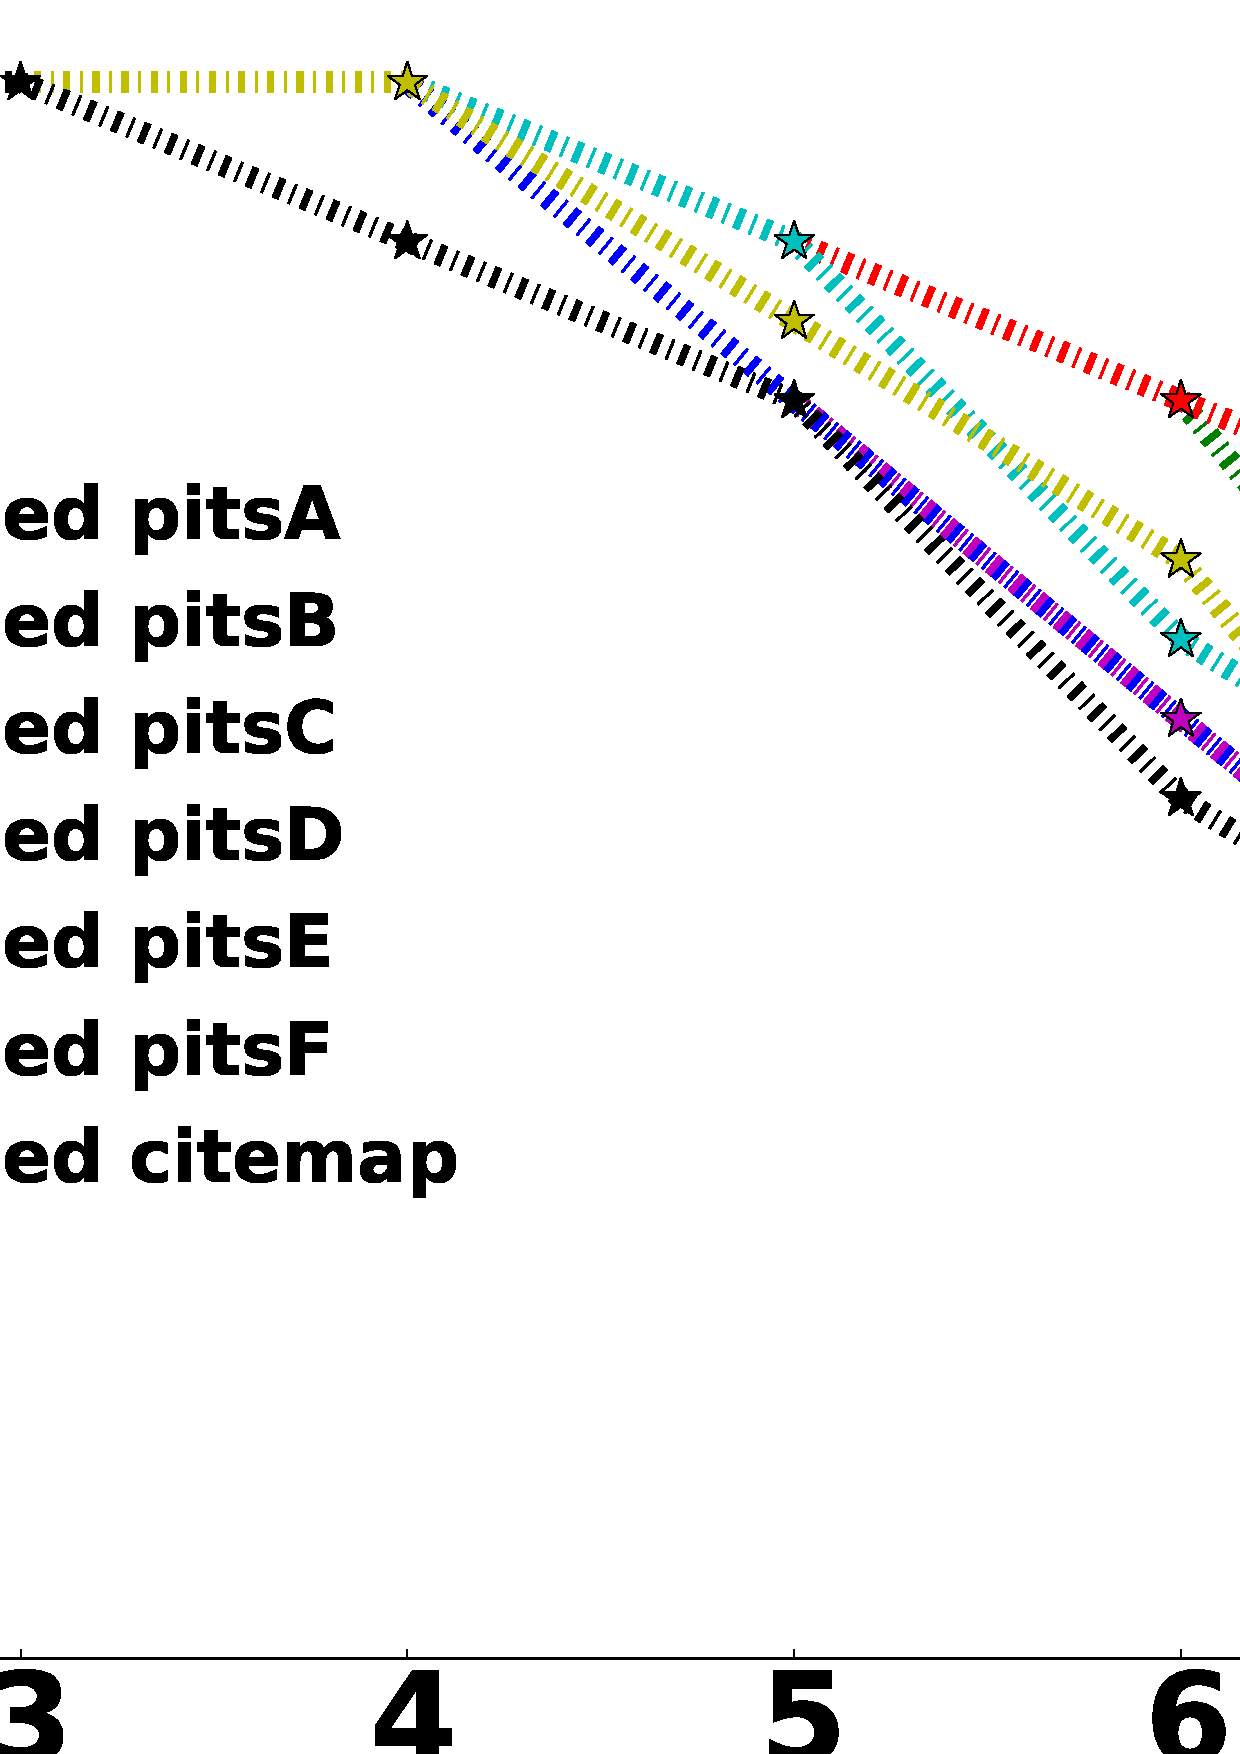
\includegraphics[width=\linewidth]{./fig/Vem_untuned.png}
  \caption{Terms vs Raw Scores between tuning and default parameters}
  \label{fig:raw_untuned}
\end{figure}
\end{center}

\subsection{\textbf{RQ2: Does tuning improve the stability scores of LDA?}}

In figure \ref{fig:raw}, x-axis represents number of terms overlap and y-axis represents the Raw scores. Different lines are for the different datasets. We can see that tuning results are either always above the default settings (untuned) or stayed the same. Since figure \ref{fig:raw} is hard to read, we have augmented the results into figure \ref{fig:delta}. In figure \ref{fig:delta}, x-axis represents number of terms overlap and y-axis represents the delta improvement which is ($tuning - untuned$) results. If the lines are above x-axis, that means tuning performed better than the untuned. Different lines are for the different datasets. It clearly shows that the answer to RQ2 is “yes” - tuning has a positive effect on stability scores. Tuning either helped it or remained the same but it never had any negative effect. The dramatic improvement started showing after 5 terms overlap. The most improvement which we observed was in PitsD dataset for 8 terms overlap of about 80\%. Delta improvement remained 0 till 5 terms overlap for most number of datasets. That's why we recommend that we shouldn't list more than 5 terms per topic, as stability starts dropping.

\begin{lesson}
Based on Figure \ref{fig:delta}, we highly recommend tuning in future LDA.
\end{lesson}

\begin{center}
\begin{figure}[!htb]
  \includegraphics[width=\linewidth]{./fig/raw_graph.eps}
  \caption{Terms vs Raw Scores between tuning and default parameters}
  \label{fig:raw}
\end{figure}
\end{center}

\begin{center}
\begin{figure}[!htb]
  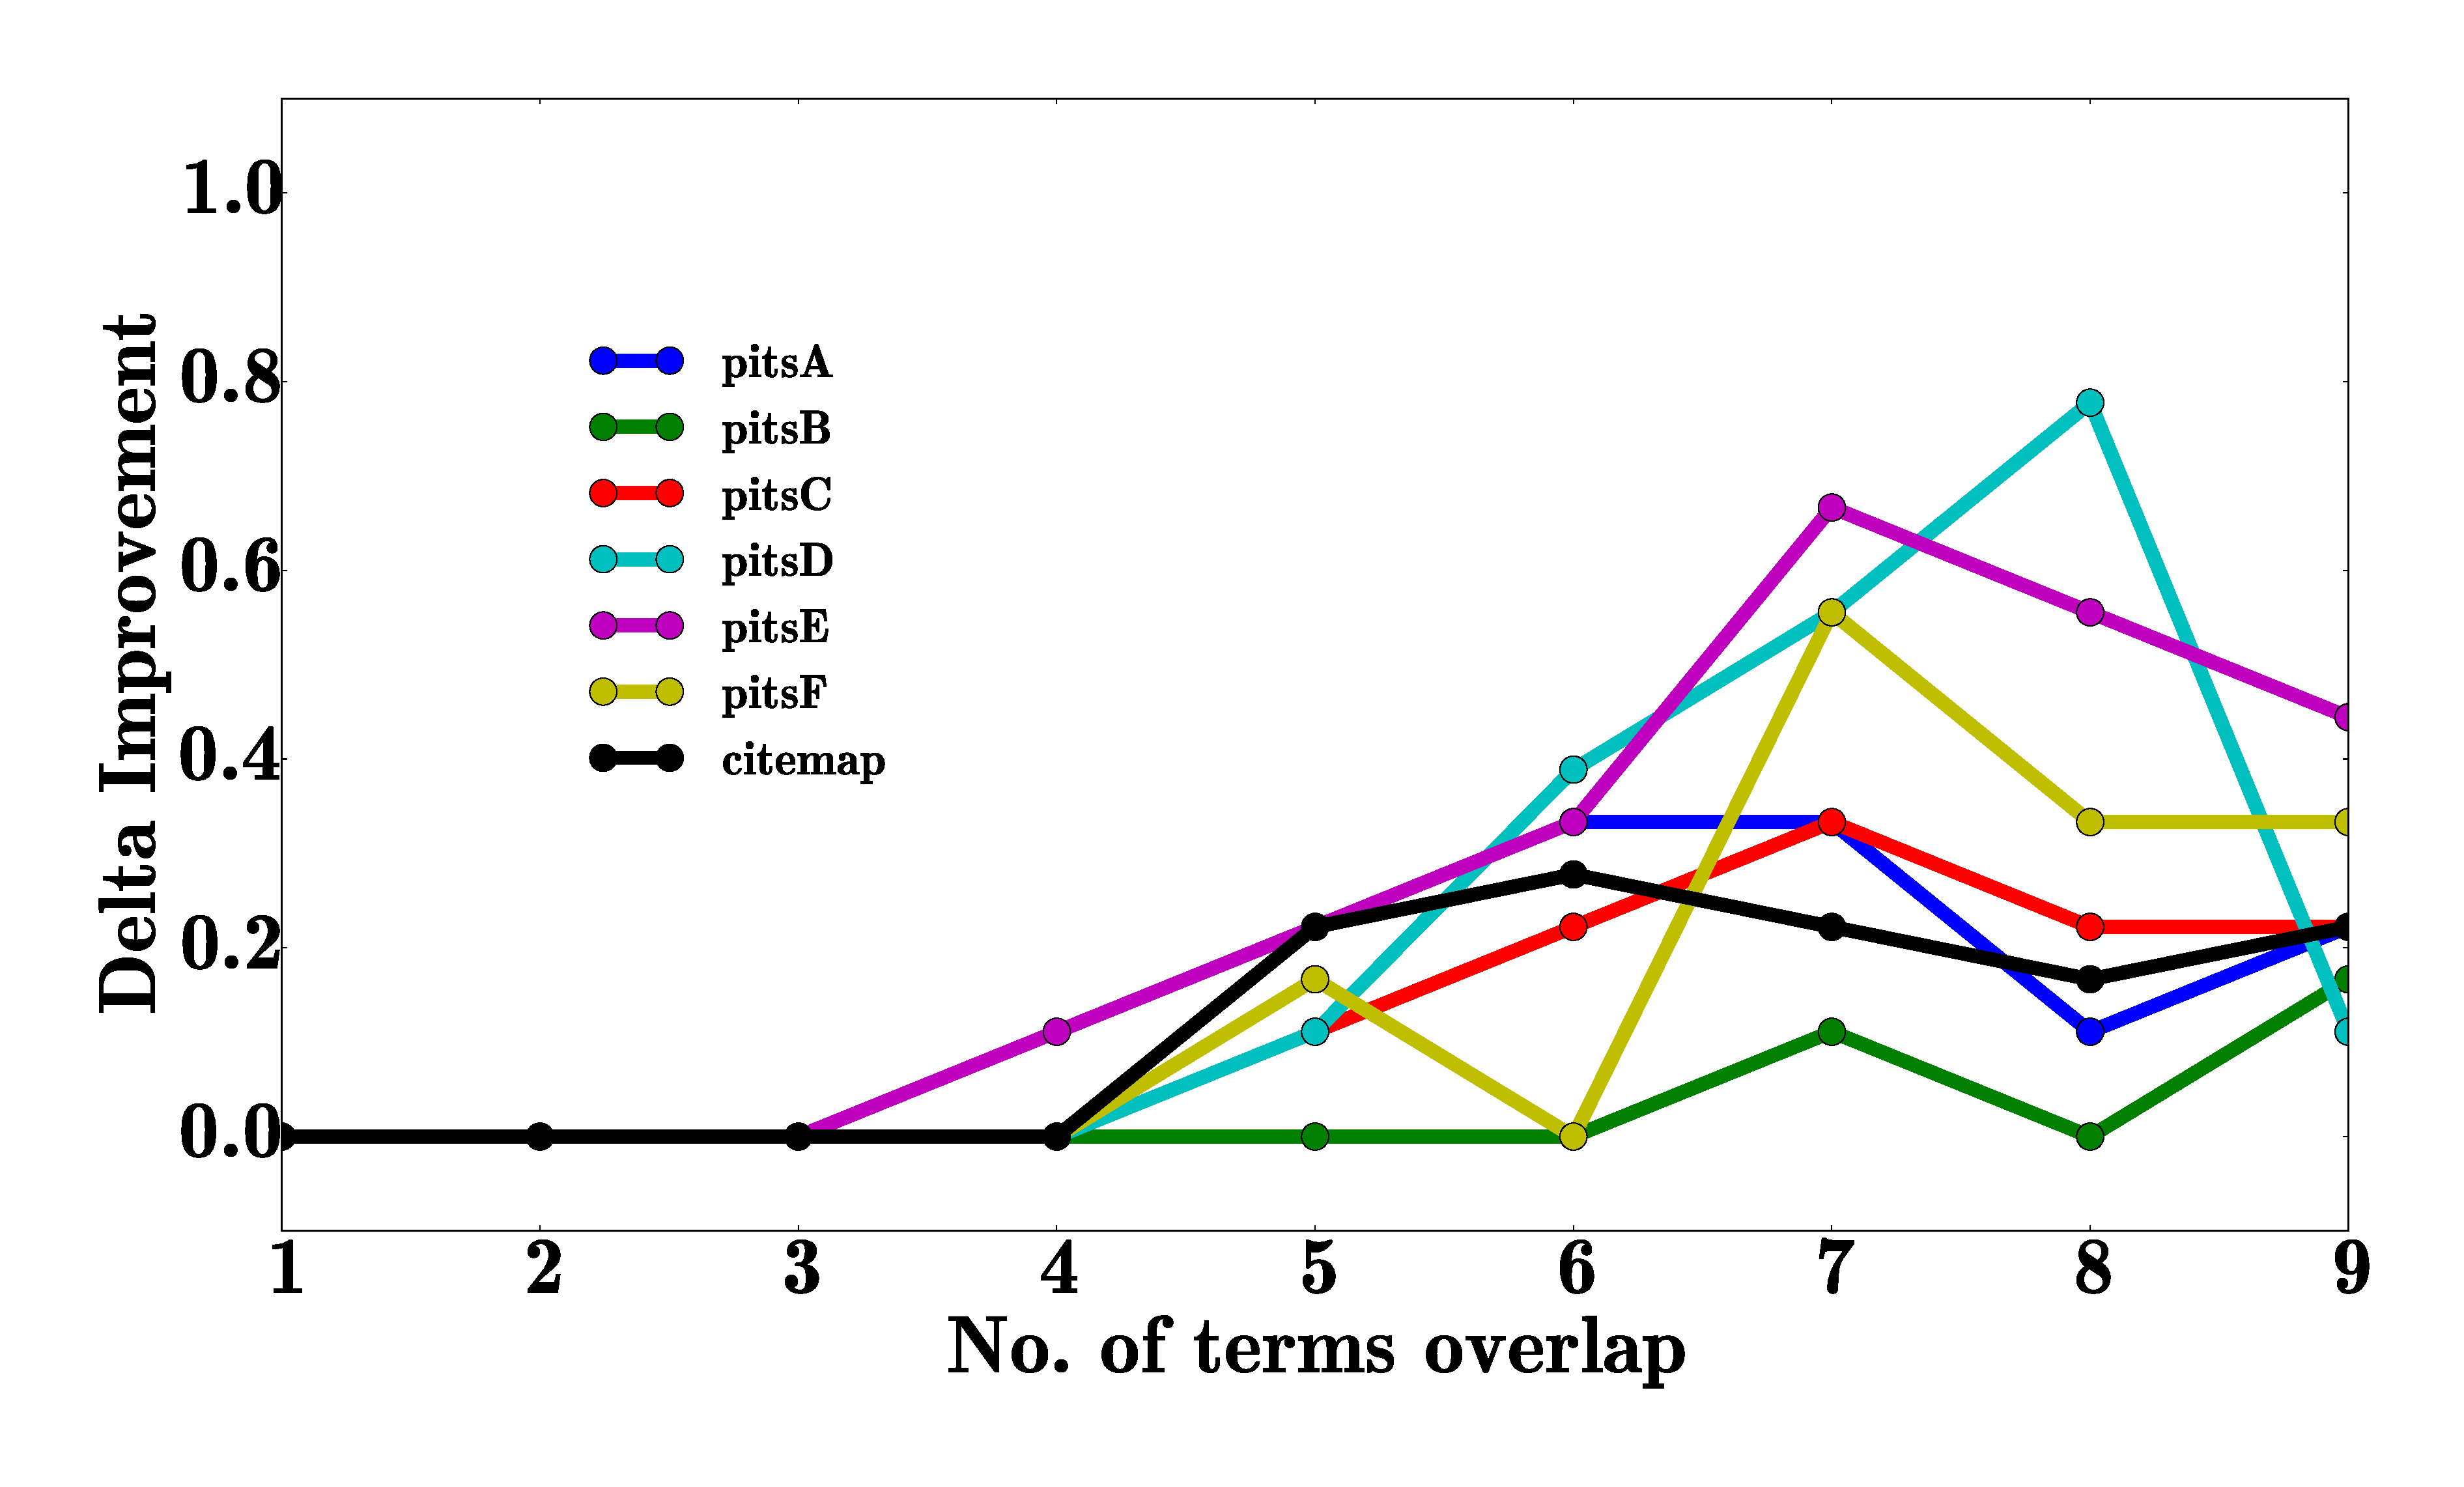
\includegraphics[width=\linewidth]{./fig/tuned_delta_vem.eps}
  \caption{Terms vs Delta Improvement between tuning and default parameters}
  \label{fig:delta}
\end{figure}
\end{center}

\subsection{\textbf{RQ3: Does different data need different configurations to make LDA stable? Does it change some predefined parameter values of lda?}}

Figures \ref{RQ3:k}, \ref{RQ3:a}, and \ref{RQ3:b}, x-axis represents different datasets and y-axis represents values of median and IQR. Each figure shows the variation in the values of number of topics (\textit{k}), alpha ($\alpha$) and beta ($\beta$). These results are for 5 terms overlap. From these figures, it clearly shows how tuning selects the different ranges of values of parameters. These figures represent a very high Median Score and as well as very high interquartile range (IQR) for different datasets. This means that tuning helped us to arrive at different sets of configurations making the topic generation more constant. In figure \ref{RQ3:k} for pitsB dataset, we are seeing 0 IQR, that means tuning helped us to find only 1 set of configurations which got us to that Stable score. We found many such similar number throughout the results. (Refer this link at \href{https://goo.gl/Nin5pV}{\textit{https://goo.gl/Nin5pV}} for elaborate results).

The other result which we found is in the citemap dataset. If we look in the spreadsheet, from Row 121-129, we see that we are getting good stable scores within 30 topic size. But in the~\cite{garousi2016citations} paper, they found that we will need a topic size of 67. Definitely, it can change predefined parameters of LDA.
We also observed the similar trend for other term overlaps as well as other sampling methods.

\begin{center}
\begin{figure}[!h]
  \includegraphics[width=\linewidth]{./fig/Parameters_variation_k.png}
  \caption{Datasets vs Parameter (k) variation}
  \label{RQ3:k}
\end{figure}
\end{center}

\begin{center}
\begin{figure}[!h]
  \includegraphics[width=\linewidth]{./fig/Parameters_variation_a.png}
  \caption{Datasets vs Parameter (alpha) variation}
  \label{RQ3:a}
\end{figure}
\end{center}

\begin{center}
\begin{figure}[!h]
  \includegraphics[width=\linewidth]{./fig/Parameters_variation_b.png}
  \caption{Datasets vs Parameter (beta) variation}
  \label{RQ3:b}
\end{figure}
\end{center}

\subsection{\textbf{RQ4: Is  tuning  easy?}}

In terms of the search space explored via tuning, it is much smaller. To see this, recall from Algorithm 2 that DE explores a Population of size np = 10. This is a very small population size since Rainer Storn (one of the inventors of DE) recommends setting np to be ten times larger than the number of parameters being optimized. We also ran experiments with different sets of F, CR, and population size (\textit{np}), and we see that it didn't change much.

We have shown results only for Citemap dataset which can be referred in Figure \ref{fig:RQ4}. For other datsets, we can refer at \href{https://goo.gl/HQNASF}{\textit{https://goo.gl/HQNASF}}. In Figure \ref{fig:RQ4}, different lines show different combinations of F, CR and Population size. F is selected either 0.3 or 0.7, and similarly CR is selected 0.3 or 0.7, and population size is selected either 10 or 30 (which is 10 times the number of parameters being optimized). These numbers are according to the original Rainer Storn~\cite{storn1997differential} recommended settings.

\begin{figure}[!htb]
  \includegraphics[width=\linewidth]{./fig/citemap.png}
  \caption{Terms vs Delta Improvement using Different settings of DE}
  \label{fig:RQ4}
\end{figure}

After reviewing the results from all the datasets, we can say that there isn't much of an improvement by using different F, CR, and Population size. So our all other experiments used $F=0.7$, $CR=0.3$ and $Pop size = 10$.

\subsection{\textbf{RQ5: Is tuning impractically slow?}}

Figure \ref{RQ5 Gibbs} and \ref{RQ5 VEM}, x-axis represents different datasets and y-axis represents the runtimes in seconds ($Log_{10}$). From the table \ref{tb:tablename1}, we will show that we just need 300 evaluations to do tuning. Using this criteria, we can see that tuning runtimes is only about 5 times the runtimes without tuning. Figure \ref{RQ5 Gibbs} is with Gibbs implemented in Python, and Figure \ref{RQ5 VEM} is with VEM implemented in Python.

\begin{center}
\begin{figure}[!h]
  \includegraphics[width=\linewidth]{./fig/Run_gibbs_sci.png}
  \caption{Gibbs: Datasets vs Runtimes}
  \label{RQ5 Gibbs}
\end{figure}
\end{center}

\begin{center}
\begin{figure}[!h]
  \includegraphics[width=\linewidth]{./fig/Run_VEM_sci.png}
  \caption{VEM: Datasets vs Runtimes}
  \label{RQ5 VEM}
\end{figure}
\end{center}

\subsection{\textbf{RQ6: Should data miners be used “off-the-shelf” with their  default  tunings?}}

From figures \ref{RQ3:k}, \ref{RQ3:a}, and \ref{RQ3:b}, we can easily see that for different datasets, we need different parameters. Such large IQRs show that we get quite varied ranges of parameters. Hence, we answer RQ6 as “no” since, to achieve the improvements seen in this paper, tuning has to be repeated whenever the goals or data sets are changed. Given this requirement to repeatedly run tuning, it is fortunate that (as shown above) tuning is so easy and so fast.

\section{Threats to Validity}
\label{sect: validity}

\textit{\textbf{Is it a quirk of the implementation?}} This instability problem remained the same across any implementation of LDA. Figure \ref{python_spark}, is with VEM method implemented in Spark. In this figure, x-axis represents different term overlaps and y-axis represents the raw stability scores. Dashed lines represents the untuned results and the solid lines represents the tuned results. We can see that tuning helped in achieving stable topic generation. The results of other datasets, can be referred at \href{https://goo.gl/UVaql1}{\textit{https://goo.gl/UVaql1}}. So it is not a quirk of implementation.

\begin{figure}[!h]
  \captionsetup{justification=centering}
  \includegraphics[width=\linewidth]{./fig/spark.png}
  \caption{Spark Results}
  \label{python_spark}
\end{figure}

\textit{\textbf{Is it a quirk of the sampling method used?}} In Figure \ref{gibbs_vem}, dashed lines represents the Gibbs implementation and solid line represents the tradition VEM method. The y-axis represents the delta improvement between tuning and untuned results. We can see that even after 5 terms, the stability score went down in both Gibbs Sampling and VEM. We also saw the same magnitude of improvements. So it is not a quirk of a particular sampling method. Here results of only 3 datasets are shown. For other datasets, results can be referred at \href{https://goo.gl/faYAcg}{\textit{https://goo.gl/faYAcg}}. So it is not a quirk of implementation.

\begin{figure}[!h]
  \captionsetup{justification=centering}
  \includegraphics[width=\linewidth]{./fig/gibbs_vem1.png}
  \caption{GIBBS vs VEM}
  \label{gibbs_vem}
\end{figure}


\textit{\textbf{Terminating criteria for DE}} From table III, we can see that after 300 evaluations, there was no improvement in the stability scores across all the datasets and it stayed the same.

\begin{table}[H]
\begin{center}
\begin{tabular}{|c|c|c|c|c|}
\hline 
\textbf{Datasets\textbackslash Evaluations} & \textbf{100} & \textbf{200} & \textbf{300} & \textbf{400} \\[0.5ex]
\hline
PitsA & 0.9 & 0.9 & 1.0 & 1.0\\ [0.5ex]
\hline
PitsB & 0.9 & 0.9 & 0.9 & 1.0 \\ [0.5ex]
\hline
PitsC & 0.9 & 1.0 & 1.0 & 1.0\\ [0.5ex]
\hline
PitsD & 0.9 & 1.0 & 1.0 & 1.0\\ [0.5ex]
\hline
PitsE & 0.9 & 0.9 & 1.0 & 1.0\\[0.5ex]
\hline
PitsF & 0.9 & 0.9 & 0.9 & 0.9\\[0.5ex]
\hline
Ciemap & 0.67 & 0.67 & 0.77 & 0.77\\[0.5ex]
\hline
Stackoverflow & 0.6 & 0.7 & 0.8 & 0.8\\[0.5ex]
\hline
\end{tabular}
\end{center}
\caption{Evaluations vs Stability Scores}
\label{tb:tablename1}
\end{table}

\section{Conclusion and Future Work}

Our exploration of the six research questions listed in the introduction shows that when doing topic modeling, analytics without parameter tuning are considered harmful and misleading. As more data getting generated day by day, it is really necessary to do accurate topic modeling. Now, with the help of tuning, we can generate stable topics to quite a good extent. Now we can delve into prior papers to improve their work. We can use the more stable LDA to find features and fed into a classifer to get improved precision and recall~\cite{chen2016topic,restificar2012inferring}

This paper showed that tuning improved the stability scores of LDA, sometimes the improvement is quite dramatic (about 80\%). This paper also highlighted that we can now select the right set of parameters for different datasets to get stable topics. This paper combined with Wei et al.~\cite{fu2016tuning} suggests that data miners should not be used off-the-shell with their default tunings.

As to future work, it is now important to explore the implications of these stable topics generated by LDA in a product development. We can now actually work with other workarounds mentioned in the section \ref{sub:supervised} with classified datasets. To improve stability, we can even try to improve the actual clusters to get better results.

This paper just investigated on stability of LDA using one optimizer. Hence, we can make no claim that DE is the best optimizer for all data miners. Rather, our point is that there exists at least some learners whose performance can be dramatically improved by at least one simple optimization scheme. And there are already claims of other unstable data miners like Decision Tree Learning, Neural Networks, and Bayesian Learning~\cite{zhang2005machine} where optimizers can mitigate instability into all these miners. We also hope that this work inspires much future work as this community develops and debugs best practices for tuning software analytics.


% Can use something like this to put references on a page
% by themselves when using endfloat and the captionsoff option.
\bibliographystyle{abbrv}
\medskip
\bibliography{sigproc}


% that's all folks
\end{document}


